\section{Phase-Scoped Implementation and Qualification (RQ2)}
\label{sec:repair}
\subsection{Constraining attention while retaining batched work}
The RTX design targets the attention graph rather than serializing the whole network. An initial implementation builds one non-flash Qwen3 attention subgraph per query and concatenates the results. The later query-batch implementation represents query columns in the ggml batch dimension, allowing existing operations to process them in parallel while preserving one-column query structure. Projection, output projection and feed-forward computation remain batched (Figure~\ref{fig:architecture}B).

After the existing query/key/value permutations, the supported single-KV-stream query has dimensions $(d,q,h,1)$. A \texttt{ggml\_view\_4d} reinterprets it as $(d,1,h,q)$, preserving the source strides and assigning the original query-column stride to the new batch axis. Shared K/V broadcast across query batches; the mask view changes from $(n_{\mathrm{KV}},q,1,1)$ to $(n_{\mathrm{KV}},1,1,q)$. Existing key-query multiplication, softmax, value multiplication and contiguous recombination perform attention. The design retains the tested scalar-query computation structure locally while preserving parallel work elsewhere; it adds no new backend arithmetic.

Implementation guards admit Qwen3 non-flash attention, one KV stream and compatible mask dimensions, with no attention bias, sinks or MLA value projection. The initial limit is four queries; a later width build extends the admitted graph to eight. Native qualification is required within those guards, and unsupported model graphs, precisions or backends inherit no preservation claim.

\subsection{Phase dispatch and graph reuse are part of the implementation}
The transformation must be active in the intended phase, including when diagnostic capture is disabled. A process-fixed mask and thread-local guard select target prefill/continuation bits 1/2 and draft prefill/continuation bits 4/8 (Figure~\ref{fig:architecture}C). The guard restores the prior active state on exit and executes before the capture-disabled fast path returns to native decoding. Diagnostic settings therefore cannot silently bypass the constraint.

The active query-batch flag is copied into graph parameters and context. Reuse is rejected if it differs from the cached topology key, preventing a phase-layout mismatch even when ordinary microbatch fields agree. A new prompt resets the phase to prefill. Role and phase therefore control graph construction and reuse directly.

Qualification checks captured multi-query nodes and capture-on/off behavior; paid capture-off sessions omit observer metadata and forced witness synchronization. The optional target-state-move branch is inactive in the expansion configuration. The measured candidate charges native drafting, verification and reconciliation without that transplant. Implementation details and timer boundaries are retained in Supplement \S S3.1.

\subsection{The finite phase family}
The factorial tests which phases require the query-batch constraint in this implementation. Figure~\ref{fig:phase}A tests all 16 masks at $k=3$/UB4 on four exposed HumanEval probes, twice each: 128 requests. Outputs and stop boundaries are repeat-stable. Masks 3, 7, 11 and 15 pass the complete panel. /15 and /31 pass every mask, /25 needs at least one target-phase bit, and /18 needs both; draft bits do not change this pattern.

\begin{figure*}[t]
\centering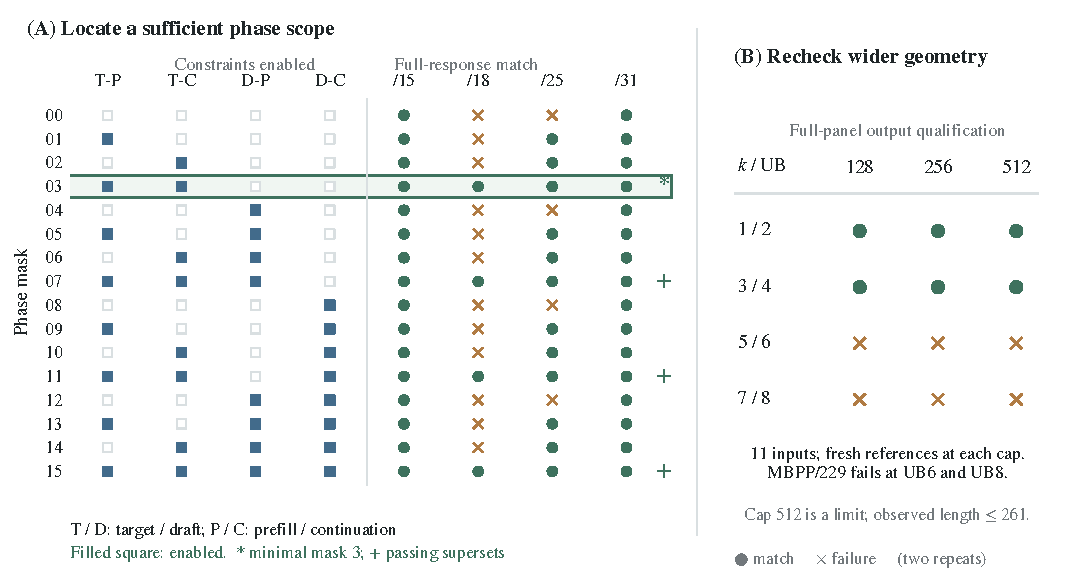
\includegraphics[width=\linewidth]{figures/figure_3_phase_matrix.pdf}
\caption{Qualification of phase scope and geometry. (A) All 16 masks at $k=3$, UB4 and cap128 on four HumanEval probes, with two repetitions (128 requests). Filled squares enable constraints; circles indicate full-response matches and crosses failures. Passing masks are 3/7/11/15; mask 3 is inclusion-minimal within this four-switch family. (B) A separate 11-input panel changes $k$ and UB jointly at caps128/256/512, using fresh scalar references and two repeats. MBPP/229 fails at UB6/8 while matched controls pass. Actual output length reaches at most 261; the earlier HE/18 target-only failure is outside this panel.}
\label{fig:phase}
\end{figure*}

Mask 3 alone has no passing strict subset, making it inclusion-minimal in the tested four-switch family. This selects a sufficient target-phase scope, not a universal requirement on every input or implementation. Acceptance, cache ownership and stopping still need to preserve the transaction. The factorial also uses different geometry from the earlier UB2/UB1 intervention, so /15's all-mask agreement does not negate that path effect.

A smaller scope need not be faster. In a separate 19-task, six-repetition cost panel, mask 3 gives $1.278\times$ generation and $1.113\times$ request speed against matched target-only. Removing draft constraints from mask 15 adds only $1.004\times$ generation speed, with descriptive interval $[0.998,1.009]$, below the frozen $1.03\times$ extra-generation gate. The later 24-input expansion gives $1.015\times$ over mask 15. Scope selection therefore follows qualification, with its cost assessed separately.

\subsection{Frozen inputs and geometry boundaries}
The frozen mask-3/$k=3$/UB4 recipe qualifies all 96 candidate responses on the 24-input expansion. Matched target-only and mask-15 speculation also qualify. This extends the repair from exposed probes to a separately frozen panel, within the same model family and configuration.

Figure~\ref{fig:phase}B tests the geometry boundary on an independent 11-input panel at $(k,\mathrm{UB})=(1,2),(3,4),(5,6),(7,8)$ and caps128/256/512, using fresh scalar references and two repeats. The first two pairs qualify; MBPP/229 fails at both wider pairs across all caps and repetitions while matched controls pass. The earlier HumanEval/18 wide target-only failure remains a separate boundary outside this denominator. The longest observed reference has 261 IDs, so cap512 is a limit rather than evidence of a 512-token trajectory.

At MBPP/229's common 47-token prefix, crossing naturally retained ordinary and constrained states under two current UB6 layouts changes the EOG decision with the donor. Current layout changes continuous scores without a separate discrete flip; four own-path shams pass. This local retained-state effect explains why changing only the current layout at that boundary is insufficient, without identifying a unique cause of all width failures. Two cap contexts repeat one task boundary. The joint $k$/UB sweep remains distinct from the fixed-UB draft-width cost experiment in Section~\ref{sec:cost}.

\subsection{A separate B570 implementation and qualification scope}
The B570 candidate uses a different control interface: it forms target state with the ordinary prompt caller and output reservation, samples the pending token once, then binds continuation from UB128 to UB1 in the same context and live sampler. A private API synchronizes, changes capacity and requests scheduler reservation under a frozen context/batch/sequence contract. Instrumented checks compare serialized KV across binding; paid capture-off requests omit witness readbacks. The existing $k=2$, draft-UB1 accept/bonus/rollback loop remains.

The candidate qualifies 12 development requests, 112 requests on 56 exposed inputs and 30 requests on 15 project-unused inputs under its endpoint contract. It removes the old second context and three witness readbacks but does not implement the RTX query-layout transformation. Earlier B570 repair produced a local long-panel gain yet failed MBPP/72 on a new-input panel and five UB2 alternatives (Supplement \S S5.1). The later same-context binding provides a separately qualified repair whose cost is assessed in the following comparisons.
